\def\mytitle{CIRCLE ASSIGNMENT}
\def\myauthor{Somisetty Kedareswari}
\def\contact{mail2kedari@gmail.com}
\def\mymodule{Future Wireless Communication (FWC)}
\documentclass[10pt, a4paper]{article}
\usepackage[a4paper,outer=1.5cm,inner=1.5cm,top=1.75cm,bottom=1.5cm]{geometry}
\twocolumn
\usepackage{graphicx}
\graphicspath{{./images/}}
\usepackage[colorlinks,linkcolor={black},citecolor={blue!80!black},urlcolor={blue!80!black}]{hyperref}
\usepackage[parfill]{parskip}
\usepackage{lmodern}
\usepackage{tikz}
	\usepackage{physics}
%\documentclass[tikz, border=2mm]{standalone}
%\usepackage{karnaugh-map}
%\documentclass{article}
\usepackage{tabularx}
%\usepackage{circuitikz}
\usepackage{enumitem}
\usetikzlibrary{calc}
\usepackage{amsmath}
\usepackage{amssymb}
\renewcommand*\familydefault{\sfdefault}
\usepackage{watermark}
\usepackage{lipsum}
\usepackage{xcolor}
\usepackage{listings}
\usepackage{float}
\usepackage{titlesec}
\providecommand{\mtx}[1]{\mathbf{#1}}
\titlespacing{\subsection}{1pt}{\parskip}{3pt}
\titlespacing{\subsubsection}{0pt}{\parskip}{-\parskip}
\titlespacing{\paragraph}{0pt}{\parskip}{\parskip}
\newcommand{\figuremacro}[5]{
    \begin{figure}[#1]
        \centering
        \includegraphics[width=#5\columnwidth]{#2}
        \caption[#3]{\textbf{#3}#4}
        \label{fig:#2}
    \end{figure}
}

\newcommand{\myvec}[1]{\ensuremath{\begin{pmatrix}#1\end{pmatrix}}}
\let\vec\mathbf
\lstset{
frame=single, 
breaklines=true,
columns=fullflexible
}
\title{\mytitle}
\author{\myauthor\hspace{1em}\\\contact\\FWC22049\hspace{6.5em}IITH\hspace{0.5em}\mymodule\hspace{6em}Assignment}
\begin{document}
	\maketitle
	\tableofcontents
   \section{Problem}
 Let C be the circle with centre $\myvec{0 \\0}$ and radius 3 units. Find the equation of the locus of the mid-points of the chords which subtend an angle of $\frac{2\pi}{3}$ at its center.
\section{Construction}
  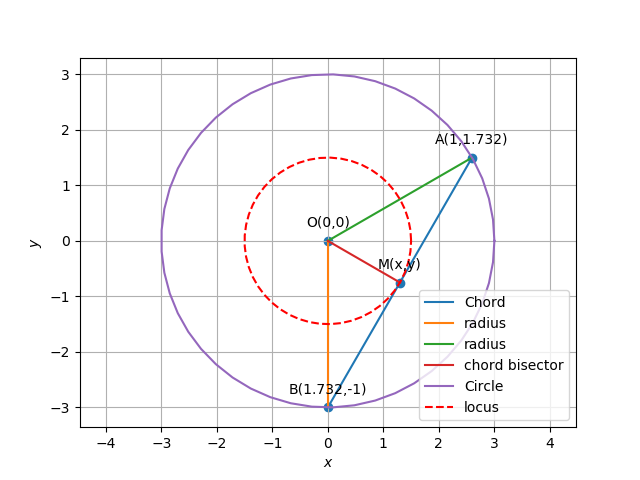
\includegraphics[scale=0.4]{circle.png}
  	\begin{center}
  Figure of construction
  	\end{center}
  \section{Solution}
Circle equation : $x^2+y^2=9$\\
The standard equation of the conics is given as :
\begin{align}
\vec{x}^{\top}\vec{V}\vec{x}+2\vec{u}^{\top}\vec{x}+f=0
\end{align}
The given circle  can be expressed as conics with \\parameters
\begin{align}
	\vec{V} &= \vec{I}, \vec{u} = -\myvec{0 \\0}, f = -9
	\end{align}

	Radius and Centre are
	\begin{align}
	r &=\sqrt{{\vec{u}^{\top}\vec{u}}-f },\vec{O}=-u
    \end{align}
\begin{equation}
  r=3 
\end{equation}
Angle between A and B is cos$\theta$ = $\frac{\vec{(A)}^{\top}\vec{B}}{||A|| ||B||}$ \\
\centering cos$120^{\circ}$ = $\frac{\vec{(A)}^{\top}\vec{B}}{9}$
\begin{align}
    \vec{(A)}^{\top}\vec{B}=\frac{-9}{2}
\end{align}\\
Let $\vec{R}$ is the rotation matrix of given circle  \\\vspace{1mm}
\begin{align}
 \vec{R} = \myvec{-0.5 & -0.866 \\0.866 & 0.5}
\end{align}

Let $\vec{B}$ be the another end point of chord \\\vspace{1mm}
\begin{align}
    \vec{B} = RA
\end{align}
Let $\vec{M}$ be th mid point of chord of the circle
\begin{align}
    \vec{M} = \frac{A+B}{2}
\end{align}
\begin{align}
     \vec{M} = \frac{A+RA}{2}
\end{align}
\begin{align}
     \vec{M} = \frac{A(I+R)}{2}
\end{align}
\begin{align}
     \vec{A} =\vec{2M[I+R]}^{-1}
\end{align}

STEPS TO FIND THE LOCUS OF THE MIDPOINT OF CHORD OF THE CIRCLE:\\
By substituting A value in quadratic form of the circle we get
\begin{align}
[\vec{2M(I+R)}^{-1}]^{\top}[\vec{2M(I+R)}^{-1}]+2[\vec{2M(I+R)}^{-1}]\myvec{0 & 0}-9=0
\end{align}
where
\begin{align}
	\vec{(I+R)}^{-1}=\myvec{0.5& 0.86 \\-0.86 & 0.5}
\end{align}
Let p be the midpoint of chord of the circle
\begin{align}
\vec{M}=\myvec{x\\y}
\end{align}

Therefore
\begin{align}
[\vec{2M(I+R)}^{-1}]^{\top}=\myvec{x+1.72y\\-1.72x+y}
\end{align}
And
\begin{align}
[\vec{2M(I+R)}^{-1}]=\myvec{x+1.72y & -1.72x+y}
\end{align}
Now the quadratic equation of given circle becomes
\begin{align}
\myvec{x+1.72y\\-1.72x+y}^{\top}\myvec{x+1.72y\\-1.72x+y}+2\myvec{x+1.72y\\-1.72x+y}\myvec{0 \\0}^{\top}-9=0
\end{align}
\begin{equation}
   (x+1.72y)^2+(-1.72x+y)^2=9
\end{equation}

\begin{equation}
   x^2+3y^2-2xy+3x^2+y^2+2xy=9
\end{equation}

\begin{equation}
   4x^2+4y^2=9
\end{equation}
 FINALLY LOCUS OF MIDPOINT OF  CHORD OF THE  GIVEN CIRCLE:\\
\begin{equation}
   \vec{x^2}+\vec{y^2}=\vec{\frac{9}{4}}
\end{equation}
The quadratic form of locus of the given circle
\begin{align}
\vec{x}^{\top}\vec{V}\vec{x}+2\vec{u}^{\top}\vec{x}+f=0
\end{align}
The given circle  can be expressed as conics with \\parameters
\begin{align}
	\vec{V} &= \vec{I}, \vec{u} = -\myvec{0 \\0}, f = -9
	\end{align}

	Radius and Centre are
	\begin{align}
	r &=\sqrt{{\vec{u}^{\top}\vec{u}}-f },\vec{O}=-u
    \end{align}
\begin{equation}
  r=\sqrt{3}
\end{equation}

\textbf{termux commands :}
\begin{lstlisting}
bash mat2.sh............using shell command
\end{lstlisting}
\begin{center}
Below python code realizes the above construction :
\fbox{\parbox{8.5cm}{\url{https://github.com/kedareswari200/fwc-module1/blob/Matri_Circle/cir.py}}}
\end{center}
\end{document}
=======
